\subsection{Hauptprogramm State Machine}\label{subsec:State_Machine}
Abbildung bla zeigt die Initialisierung und den Hauptprogrammfluss der Software.
\begin{figure}[h]
	\centering
	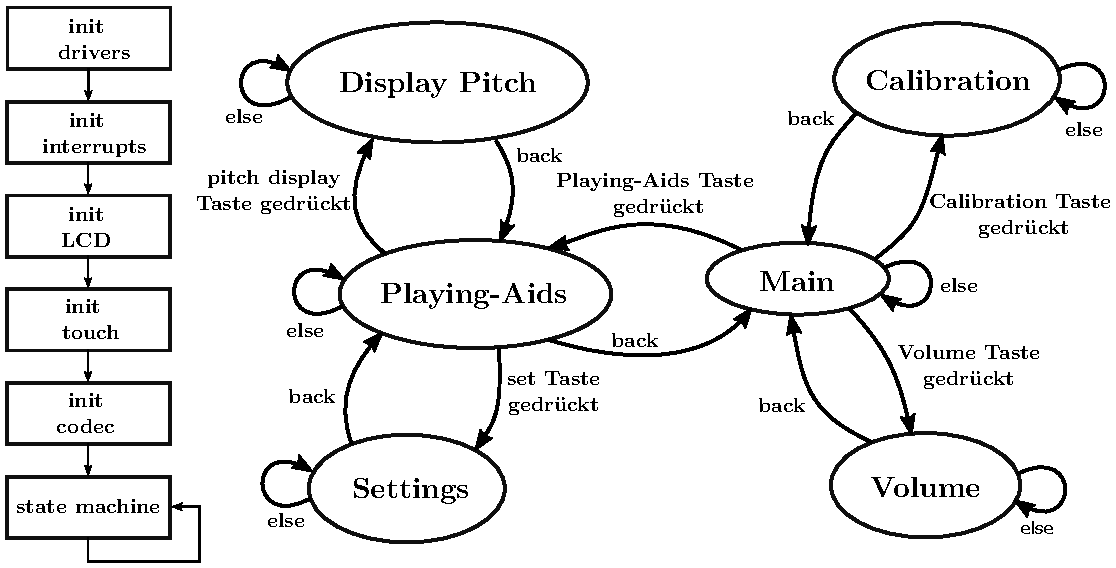
\includegraphics[width=\textwidth]{state_machine.pdf}
	\caption{State Machine und Initailisierung.}
	\label{img:Blockschaltbild_digital}
\end{figure}

In der Initialisierung werden als erstes alle Treiber, der Touch, das LCD, und der Codec, und  konfiguriert. Anschlissend wird in einer Endlosschlaufe die state machine aufgerufen.

\textbf{Main}:
Dies ist der erste State nach dem Initialisierungsvorgang. In diesem State wird gewartet bis der Benutzer einer der drei in Abbildung bla gezeigten Tasten drückt. Danach wird je nachdem welcher Taster betätigt wurde in den entsprechende State gewechselt. 
 
\textbf{Calibration}:
Im Calibration State wird der Benutzer gebeten seine Hände in die Nähe der Antenne zu halten.
Nach zwei Sekunden wird die Kalibrierung gestartet. Sobald die Kalibrierung abgeschlossen ist kann der Benutzer über den \textbf{\textit{back}} Taste zurück in den Main State gelangen.  

\textbf{Volume}:
In diesem State kann der Benutzer die Lautstärke ändern und die Volume Antenne aktivieren und deaktivieren. Die Lautstärke kann in 10 verschiedene Pegel eingestellt werden. Dies geschieht mithilfe der in Abbildung bla gezeigten \textbf{\textit{+}} und \textbf{\textit{-}} Tasten. Beim betätigen der \textbf{\textit{vol antenna}} taste wird die Volume Antenne je nach aktuellem Zustand deaktiviert oder aktiviert. Mit dem betätigen der \textbf{\textit{back}} Taste gelangt der Benutzer in den Main State.
 
\textbf{Play Help}:
Im State Play Help kann mit der\textbf{\textit{Glissando on}} Taste der Glissando Effekt akieviert und deaktiviert werden. Über die \textbf{\textit{Set}} Taste gelangt man in den State Settings. Durch betätigen des \textbf{\textit{display pitch}} Taste wird in den State Pitch Display gewechselt.  Mit dem betätigen der \textbf{\textit{back}} Taste gelangt der Benutzer in den Main State.

\textbf{Settings}:
Im Settings State können Einstellungen zum Glissando Effekt gemacht werden. Das Delay des Glissando Effekts kann in 10 Stufen eingestellt werden. Zudem kann mit dem Taster \textbf{\textit{penta}} zwischen der Pentatonischer und der normalen Tonleiter gewechselt werden. Mit dem betätigen der \textbf{\textit{back}} Taste gelangt der Benutzer in den Main State.

\textbf{Pitch Display}:
Im Pitch Display State kann der Benutzer sehen welcher Ton gespielt wird. Ist die Pentatonische Tonleiter aktiv wird angezeigt wie weit man von einem Ton entfernt ist. Falls die normale Tonleiter aktiv ist wird der Ton angezeigt bei welchem man sich am nächsten befindet.

